\section{Data Conditioning}
\label{sec:conditioning}
% Mention approximants used for the template bank? or instead mentioned ranges
% of template bank parameter space?
\lorena{The training and testing datasets represent $\sim 200,000$ binary
systems comprised of BBHs, BNSs, and NSBHs. The injections of these systems 
come from the Mock Data Challenge (MDC) conducted during LIGO's second 
observing run (O2) and are recovered using \texttt{GstLAL}, a low-latency 
detection pipeline. The data is divided into a training/testing breakdown 
of $70\%/30\%$. Regression is applied to four features, namely the 
initial masses $m_1$ and $m_2$ and initial spin magnitudes $\chi_1$ and 
$\chi_2$. The training dataset has mass ranges $m_1 =  [1.02, 116]$ and 
$m_2 =  [0.81, 81]$ and spin ranges $\chi_{1,2} =  [-0.99, 0.99]$, as 
shown in Fig.~\ref{parameter_space}.}

\begin{figure}
	\centering
	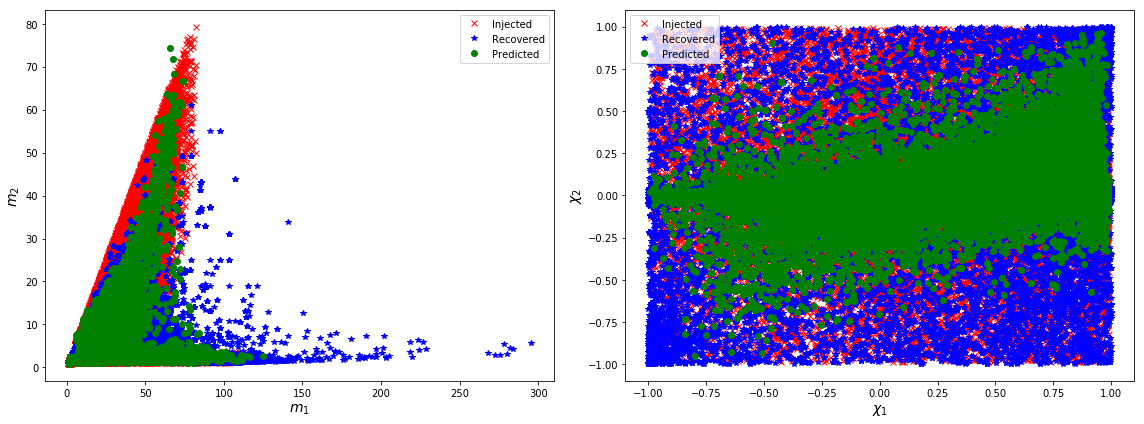
\includegraphics[width=0.45\textwidth]{m1m2_chi1chi2_comparison.png}
    \caption{\lorena{The $m_1$-$m_2$ (left) and $\chi_1$-$\chi_2$ (right) parameter space 
		of injections is shown in red, the recovered
  		values from matched-filtering are in blue, and the predicted values from 
        regression are in green.}}
	\label{parameter_space}
\end{figure}

\lorena{ML algorithms require the data to be standardized, i.e. have a zero
mean and unit variance. However, before standardizing the data we take an 
additional step to ensure astrophysical values from the predictions. In other 
words, a prediction without proper data conditioning can result in negative
masses and spin magnitudes greater than one. To avoid this, we first map the 
data to be in the $(0,1)$ range by solving a simple, linear system of equations 
separately for the masses and the spins. We, then, transform our data using a 
sigmoid function so that the values map between $- \infty$ and $+ \infty$. It
is only at this point that the data is ready to be standardized and fed into
GPR and NN. Once the algorithm gives us the predicted data, or the corrected
paramters estimates, the reverse process is applied, i.e., the data is scaled 
back from standardization, exponentiated, and mapped back to from $(0,1)$ to
physical values.}
